\documentclass[12pt, twoside]{report}
\usepackage[utf8]{inputenc}
\usepackage[T1]{fontenc}
\usepackage[spanish]{babel}
\usepackage[letterpaper,width=150mm,top=25mm,bottom=25mm,bindingoffset=6mm]{geometry}
\usepackage{utopia}
\usepackage{pdfpages}
\usepackage{hyperref}
\usepackage{booktabs}
\usepackage[font=small,labelfont=bf]{caption}
%\hypersetup{
%    colorlinks=true,
%    linkcolor=blue,
%    filecolor=magenta,      
%    urlcolor=cyan
%}



\usepackage{setspace}
\doublespacing

%\usepackage{fancyhdr}
%\pagestyle{fancy}

\usepackage{graphicx}
\graphicspath{ {imagenes/} }

\usepackage[]{gitinfo2}
%\renewcommand{\gitMark}{\centering{Branch: \gitBranch,@\,\gitAbbrevHash{} \textbullet{} Release:\gitReln{} (\gitAuthorIsoDate)\\ Commiter:\gitCommitterName, Head tags:\gitTags} \textbullet{} References: \gitReferences}

\setcounter{tocdepth}{4}
\setlength{\parskip}{1em}

\begin{document}

\thispagestyle{plain}
\begin{titlepage}
	\begin{center}
        {\fontsize{24}{28}\fontfamily{phv}\selectfont \textbf{Instituto Tecnológico de Costa Rica}\\}
        \vspace{1cm}
        {\fontsize{20}{24}\fontfamily{phv}\selectfont \textbf{Escuela de Ingeniería en Computación}\\}
        {\fontsize{18}{22}\fontfamily{phv}\selectfont \textbf{Programa de Maestría en Computación}\\}
        \vspace{2cm}
        {\fontsize{20}{24}\fontfamily{phv}\selectfont \textbf{Modelado y simulación de funciones en la nube en plataformas \textit{Function-as-a-Service}}}    
    
    
        \vspace{2cm}
        {\fontsize{14}{17}\fontfamily{phv}\selectfont \textbf{Propuesta de Tesis sometida a consideración del Departamento de Computación, para optar por el grado de Magíster Scientiae en Computación, con énfasis en Ciencias de la Computación
}}
        
       \vspace{1.5cm}
       {\fontsize{14}{17}\fontfamily{phv}\selectfont \textbf{Estudiante\\ Carlos Martín Flores González}} 
       
       \vspace{1cm}
       {\fontsize{14}{17}\fontfamily{phv}\selectfont \textbf{Profesor Asesor\\ Ignacio Trejos Zelaya}}
       
       \vspace{1.5cm}
       {\fontsize{14}{17}\fontfamily{phv}\selectfont \textbf{Noviembre, 2018}}                       
        
    \end{center}
\end{titlepage}

%\maketitle
\pagenumbering{roman} 
\renewcommand*\contentsname{Índice}
\tableofcontents
\listoffigures
%\listoftables

\newpage
{\footnotesize
\noindent
\texttt{
Git: \gitReferences \\
Branch: \gitBranch \\
Tag: \gitVtag \\
Release: \gitReln{} \\
Commit: \gitAbbrevHash \\
Date: \gitAuthorIsoDate \\
Author: \gitAuthorName\\
Email: \gitAuthorEmail\\
Committer: \gitCommitterName\\
Committer email: \gitCommitterEmail
}}
\newpage

\chapter{Introducción}
\pagenumbering{arabic}
Los servicios de funciones en la nube (\textit{Function-as-a-Service, FaaS}) representan una nueva tendencia de la computación en la nube en donde se permite a los desarrolladores instalar código, en forma de función, en una plataforma de servicios en la nube y en donde la infraestructura de la plataforma es responsable de la ejecución, el aprovisionamiento de recursos, monitoreo y el escalamiento automático del entorno de ejecución. El uso de recursos generalmente se mide con una precisión de milisegundos y la facturación es por usualmente 100 ms de tiempo de CPU utilizado. 

En este contexto, el ``código en forma de función'' es un código que es pequeño, sin estado, que trabaja bajo demanda y que tiene una sola responsabilidad funcional. Debido a que el desarrollador no necesita preocuparse de los aspectos operacionales de la instalación o el mantenimiento del código, la industria empezó a describir este código como uno que no necesitaba de un servidor para su ejecución, o al menos de una instalación de servidor como las utilizadas en esquemas tradicionales de desarrollo, y acuñó el término \textit{serverless} (sin servidor) para referirse a ello. 

\textit{Serverless} se utiliza entonces para describir un modelo de programación y una arquitectura en donde fragmentos de código son ejecutados en la nube sin ningún control sobre los recursos de cómputo en donde el código se ejecuta. Esto de ninguna manera es una indicación de que no hay servidores, sino simplemente que el desarrollador delega la mayoría de aspectos operacionales al proveedor de servicios en la nube. A la versión de \textit{serverless} que utiliza explícitamente funciones como unidad de instalación se le conoce como \textit{Function-as-a-Service}\cite{DBLP:journals/corr/BaldiniCCCFIMMR17}.

Aunque el modelo FaaS brinda nuevas oportunidades, también introduce nuevos retos. Uno de ellos tiene que ver con el rendimiento de la función, puesto que en este modelo solamente se conoce una parte de la historia, la del código, pero se omiten los detalles de la infraestructura que lo ejecuta. La información de esta infraestructura, su configuración y capacidades es relevante para arquitectos y diseñadores de software para lograr estimar el comportamiento de una función en plataformas FaaS. 

El problema de la estimación del rendimiento de aplicaciones en la nube, como lo son las que se ejecutan en plataformas FaaS y arquitecturas basadas en microservicios, es uno de los problemas que  está recibiendo mayor atención especialmente dentro de la comunidad de investigación en ingeniería de rendimiento de software. Se argumenta que a pesar de la importancia de contar con niveles altos de rendimiento, todavía hay una falta de enfoques de ingeniería de rendimiento que consideren de forma explícita las particularidades de los microservicios\cite{Heinrich:2017:PEM:3053600.3053653}.

Si bien, para FaaS, existen plataformas \textit{open source} por medio de las cuales se pueden obtener los detalles de la infraestructura y de esta manera lograr un mejor entendimiento acerca del rendimiento esperado, estas plataformas cuentan con arquitecturas grandes y complejas, lo cual hace que generar estimación se convierta en una tarea sumamente retadora.

En este trabajo se plantea explorar la aplicación de modelado de rendimiento de software basado en componentes para funciones que se ejecutan en ambientes FaaS. Para esto se propone utilizar una función de referencia y, a partir de esta, generar cargas de trabajo para recolectar datos de la bitácora(\textit{logs}) de ejecución y extraer un modelo a partir de ellos. Una vez que se cuente con un modelo, se procederá con su análisis y simulación a fin de evaluar si el modelo generado logra explicar el comportamiento de la función bajo las cargas de trabajo utilizadas.

Esta propuesta está organizada de la siguiente manera: en el capítulo \ref{cap:antecedentes} se presenta un marco conceptual sobre ingeniería de rendimiento de software y trabajos de investigación relacionados con ingeniería de rendimiento de software en aplicaciones en la nube, microservicios y \emph{serverless}. En el capítulo \ref{cap:problema} se define el problema a resolver. En el capítulo \ref{cap:justificacion} se proporciona una justificación del proyecto desde las perspectivas de innovación, impacto y profundidad. El objetivo general y los objetivos específicos se plantean en el capítulo \ref{cap:objetivos}. El alcance del proyecto se define en el capitulo \ref{cap:alcance}. Los entregables que se generarán a partir de esta propuesta se listan en el capítulo \ref{cap:entregables}. La metodología de trabajo se indica en el capítulo \ref{cap:metodologia}. La propuesta concluye en el capítulo \ref{cap:cronograma}, donde se presenta el cronograma de actividades.

%Los métodos de predicción de rendimiento basados en modelos permiten a los arquitectos de software evaluar el rendimiento de los sistemas de software durante las primeras etapas de desarrollo. Estos modelos de predicción se centran en los aspectos relevantes de la arquitectura y de la lógica del negocio, dejando de lado detalles de la infraestructura subyacente. Sin embargo, estos detalles son esenciales para generar predicciones de rendimiento que sean precisas.
%
%Para los ingenieros, es una práctica común simular el modelo de un artefacto antes de construirlo. Modelos de diseños de autos, circuitos electrónicos, puentes, entre otros, son simulados para entender el impacto de decisiones de diseño en varias atributos de calidad de interés como seguridad, consumo de energía o estabilidad. La habilidad de predecir las propiedades de un artefacto basado en su diseño y sin necesidad de construirlo, es una de las características centrales de una disciplina de ingeniería. A partir de esta visión, de lo que se considera una disciplina de ingeniería establecida, se podría decir entonces que la ingeniería de software es apenas una disciplina de ingeniería\cite{Reussner:2016:MSS:3036121}. Esto porque frecuentemente los ingenieros de software carecen del entendimiento del impacto de decisiones de diseño en atributos de calidad como rendimiento o confiabilidad. Como resultado, se intenta probar la calidad del software mediante costosos ciclos de prueba y error.
%
%El no entender el impacto en las decisiones de diseño puede ser costoso y riesgoso. El probar software significa que ya se ha hecho un esfuerzo en su implementación. Por ejemplo, si las pruebas revelan problemas de rendimiento, es muy probable que la arquitectura necesita ser modificada, lo que puede conllevar a costos adicionales. Estos costos surgen debido a que en sistemas de software empresarial un bajo rendimiento es principalmente el efecto de una arquitectura inadecuada que efecto de código.
%
%La ingeniería de rendimiento de software(SPE por sus siglas en inglés) es una disciplina que se centra en incorporar aspectos de rendimiento dentro del proceso de desarrollo de software, con el objetivo de entregar software confiable de acuerdo con propiedades de rendimiento particulares. Los modelos de rendimiento predictivos son una de las herramientas empleadas en SPE. Construidos en las fases tempranas del proceso de desarrollo de software, los modelos ayudan a predecir el rendimiento eventual del software y de esta forma guiar el desarrollo, para eso los modelos de predicción de rendimiento deben capturar todos los componentes relevantes del sistema.
%
%Para aplicaciones de software modernas, esto puede implicar modelar complejas capas tales como máquinas virtuales o \emph{middleware} de mensajería. Componer todos estos modelos puede resultar una tarea costosa e ineficiente. En su lugar, un modelo abstracto de la aplicación se puede construir primero y luego ir agregando los modelos de los componentes del sistema. 
%
%En este trabajo se propone la construcción de un modelo de rendimiento para un sistema que utilice \emph{middleware} orientado a mensajes con el fin de evaluar la influencia en el rendimiento de dicho sistema. Se propone evaluar esta influencia por medio de un ejemplo: tomar una aplicación de referencia con el fin de obtener sus métricas actuales de rendimiento, adaptarla para que utilice \emph{middleware} orientado a mensajes y luego medir su rendimiento y generar un modelo a partir de esto.


\chapter{Antecedentes}
\label{cap:antecedentes}
% Notas:
% Sobre originalidad: distiguir mi software del SaaS
% ======================================

\section{Marco conceptual}

\subsection{Ingeniería de rendimiento de software (\emph{Software Performance Engineering})}
Una definición comúnmente utilizada para definir ingeniería de rendimiento de software  (\emph{Software Performance Engineering} - SPE)  es la que brinda en Woodside et al. \cite{4221619}: \textit{``Ingeniería de rendimiento de software representa toda la colección de actividades de ingeniería de software y análisis relacionados utilizados a través del ciclo de desarrollo de software que están dirigidos a cumplir con los requisitos de rendimiento''}. 

De acuerdo con este mismo autor, los enfoques para ingeniería de rendimiento puede ser divididos en dos categorías: basadas en mediciones y basadas en modelos. La primera es la más común y utiliza pruebas, diagnóstico y ajustes una vez que existe un sistema en ejecución que se puede medir, es por esto que solamente puede ser utilizada conforme se va acercando el final del ciclo de desarrollo de software. Al contrario del enfoque basado en mediciones, el enfoque basado en modelos se centra en las etapas iniciales del desarrollo. Como el nombre lo indica, en este enfoque los modelos son clave para hacer predicciones cuantitativas de qué tan bien una arquitectura puede cumplir sus expectativas de rendimiento.

Se han propuesto otras clasificaciones de enfoques para SPE pero, con respecto a la evaluación de sistemas basados en componentes, en \cite{Koziolek:2010:PEC:1808359.1808729} se deja la clasificación a un lado debido a que se argumenta que la mayoría de enfoques de modelaje toman alguna medición como entrada y a la mayoría de los métodos de medición los acompaña algún modelo.

\subsubsection{Ingeniería de rendimiento basada en mediciones}
Los enfoques basados en mediciones son los que prevalencen en la industria\cite{Gooijer2011PerformanceMO} y son típicamente utilizados para verificación(¿el sistema cumple con su requisito de rendimiento?) o para localizar y arreglar \emph{hot-spots} (cuáles son las partes que tienen peor rendimiento en el sistema). La medición de rendimiento se remonta al inicio de la era de la computación, lo que ha generado una amplia gama de herramientas como generadores de carga y monitores para crear cargas de trabajo ficticias y llevar a cabo la medición de un sistema respectivamente.

Las pruebas de rendimiento aplican técnicas basadas en medición y usualmente esto es hecho luego de las pruebas funcionales o de carga. Las pruebas de carga verifican el funcionamiento de un sistema bajo cargas de trabajo pesadas, mientras que las pruebas de rendimiento son usadas para obtener datos cuantitativos de características de rendimiento, como tiempos de respuesta, \emph{throughput} y utilización de hardware para una configuración de un sistema bajo una carga de trabajo definida.

\subsubsection{Ingeniería de rendimiento por medio de modelado} 
La importancia del modelado del rendimiento está motivada por el riesgo a que se presenten problemas graves de rendimiento y la creciente complejidad de sistemas modernos, lo que hace difícil abordar los problemas de rendimiento al nivel de código\cite{Reussner:2016:MSS:3036121}. Cambios considerables en el diseño o en las arquitecturas pueden ser requeridos para mitigar los problemas de rendimiento. Por esta razón, la comunidad de investigación de modelado de rendimiento intenta luchar contra el enfoque de ``arreglar las cosas luego'' durante el proceso de desarrollo. Con la aplicación de un modelo del rendimiento de software se busca encontrar problemas de rendimiento y alternativas de diseño de manera temprana en el ciclo de desarrollo, evitando así el costo y la complejidad de un rediseño o cambios en los requerimientos.

Las herramientas de modelado de rendimiento ayudan a predecir la conducta del sistema antes que este sea construido o bien, evaluar el resultado de un cambio antes de su implementación. El modelado del rendimiento puede ser usado como una herramienta de alerta temprana durante todo el ciclo de desarrollo con mayor precisión y modelos cada vez más detallados a lo largo del proceso. Al inicio del desarrollo un modelo no puede ser validado contra un sistema real, por esto el modelo representa el conocimiento incierto del diseñador. Como consecuencia de esto el modelo hace suposiciones que no necesariamente se van a dar en el sistema real, pero que van a ser útiles para obtener una abstracción del comportamiento del sistema. En estas fases iniciales, la validación se obtiene mediante el uso del modelo, y existe el riesgo de conclusiones erróneas debido a su precisión limitada. Luego, el modelo puede ser validado contra mediciones en el sistema real (o parte de este) o prototipos y esto hace que la precisión del modelo se incremente.

En \cite{Jin:2007:PEP:1248820.1248885} se sugiere que los métodos actuales tienen que superar un número de retos antes que puedan ser aplicados en sistemas existentes que enfrentan cambios en su arquitectura o requerimientos. Primero, debe quedar claro cómo se obtienen los valores para los parámetros del modelo y cómo se pueden validar los supuestos. Estimaciones basadas en la experiencia para estos parámetros no son suficientes y mediciones en el sistema existente son necesarias para hacer predicciones precisas. Segundo, la caracterización de la carga del sistema en un entorno de producción es problemática debido a los recursos compartidos (bases de datos, hardware). Tercero, deben desarrollarse métodos para capturar parámetros del modelo dependientes de la carga. Por ejemplo un incremento en el tamaño de la base de datos probablemente incrementará las necesidades de procesador, memoria y disco en el servidor.

Técnicas comúnes de modelado incluyen redes de colas y también extensiones de estas como redes de colas en capas y varios tipos de redes de Petri, y procesos de álgebra estocástica.

\subsubsection{Modelado de Rendimiento}
En SPE, la creación y evaluación de modelos de rendimiento es un concepto clave para evaluar cuantitativamente el rendimiento del diseño de un sistema y predecir el rendimiento de otras alternativas de diseño. Un modelo de rendimiento captura el comportamiento relevante al rendimiento de un sistema para identificar el efecto de cambios en la configuración o en la carga de trabajo en el rendimiento. Permite predecir los efectos de tales cambios sin necesidad de implementación y ejecución en un ambiente de producción, que podrían ser no solamente tareas costosas sino también un desperdicio en el caso que un el hardware con el que se cuenta pruebe ser insuficiente para soportar la intensidad de la carga de trabajo.\cite{Noorshams2015_1000046750}

La forma del modelo de rendimiento puede comprender desde funciones matemáticas a formalismos de modelado estructural y modelos de simulación. Estos modelos varían en sus características clave, por ejemplo, las suposiciones de modelado de los formalismos, el esfuerzo de modelado requerido y el nivel de abstracción.

En cuanto a técnicas de simulación, a pesar que estas permiten un estudio más detallado de los sistemas que modelos analíticos, la construcción de un modelo de simulación requiere de conocimiento detallado tanto de desarrollo de software como de estadística\cite{Gooijer2011PerformanceMO}. Los modelos de simulación también requieren usualmente de mayor tiempo de desarrollo que los modelos analíticos. En \cite{4221619} se menciona que ``la construcción de un modelo de simulación es caro, algunas veces comparable con el desarrollo de un sistema, y, los modelos de simulación detallados puede tardar casi tanto en ejecutarse como el sistema''.

\subsection{Modelado y simulación de rendimiento basado en componentes}
En este enfoque, modelos clásicos de rendimiento tales como redes de colas, redes de Petri estocásticas o procesos de álgebra estócastica son aplicados para modelar y analizar el rendimiento de software basado en componentes. La ingeniería de software basada en componentes se considera un sucesor del desarrollo de software orientado a objetos, en esta los componentes de software son unidades de composición a las que se le define una especificación y una interfaz. A partir de estas, los arquitectos de software construyen e integran componentes de software entre sí, creando de esta manera sistemas más complejos.\cite{Koziolek:2010:PEC:1808359.1808729}

El reto en los modelos de rendimiento para componentes, es que el rendimiento de un componente de software en un sistema en ejecución depende del contexto en que está instlado y su perfil de uso, el cual es usualmente desconocido por el desarrollador del componente que creal el modelo de un componente individual.

\subsubsection{Rendimiento de componentes de software}
Szyperski\cite{Szyperski:2002:CSB:515228} define un componente de software como: \textit{``Un componente es una unidad de composición en aplicaciones de software, que posee un conjunto de interfaces y un conjunto de requisitos (una especificación), y que ha de poder ser desarrollado, adquirido, incorporado al sistema y compuesto con otros componentes de forma independiente, en tiempo y espacio''}. 

Los componentes de software presentan los principios de ocultación de la información y la separación de responsabilidades. Fomentan la reutilización y preparan el sistema para que se puedan efectuar cambios de partes individuales. Permiten además una división de trabajo entre los desarrolladores de componentes y los arquitectos de software, lo que reduce la complejidad de la tarea de desarrollo. Los componentes de caja negra (\emph{black-box}) solamente revelan sus interfases a los clientes, mientras que los componentes de caja blanca (\emph{white-box}) permiten ver y modificar el código fuente de la implementanción del componente como tal. Los componentes compuestos agrupan varios componentes en unidades más grandes.

\paragraph{Factores que influyen el rendimiento de un componente}
Especificar el rendimiento de componentes reutilizables es difícil porque esto no solamente va a depender de la implementación del componente, sino también del contexto en donde se encuentre instalado. Los factores que influyen en el rendimiento de los componentes son:

\begin{figure}[h]
  \centering
  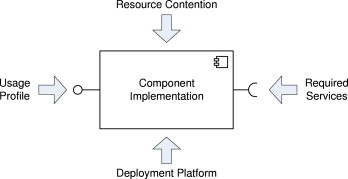
\includegraphics[width=10cm]{component-performance}
  \caption[Factores que influyen en el rendimiento de un componente]{Factores que influyen en el rendimiento de un componente. Tomado de \protect\cite{Koziolek:2010:PEC:1808359.1808729}}
  \label{fig:component-performance}
\end{figure}

\begin{itemize}
    \item \emph{Implementación del componente}: los desarrolladores pueden implementar la funcionalidad especificada en una interfaz de diferentes formas. Dos componentes pueden proporcionar el mismo servicio pero presentar tiempos de ejecución diferentes cuando se ejecutan con los mismos recursos y con las mismas entradas.
    \item \emph{Servicios requeridos}: cuando el componente $A$ invoca el servicio del componente $B$, el tiempo de ejecución de $B$ suma al tiempo de ejecución de $A$. Por lo tanto, el tiempo total de ejecución de un componente depende del tiempo de ejecución de los otros componentes/servicios que necesita.
    \item \emph{Plataforma de instalación}: los arquitectos de software instalan un componente de software en diferentes plataformas. Una plataforma de instalación puede incluir varias capas de software (como por ejemplo contenedores de componentes o máquinar virtuales) y hardware (procesador, dispositivos de almacenamiento y red, etc)
    \item \emph{Perfil de uso}: clientes pueden invocar los servicios del componente con diferentes parámetros de entrada. El tiempo de ejecución de un servicio puede cambiar dependiendo de los valores de lo parámetros de entrada.
    \item \emph{Contención de recursos}: un componente de software típicamente no se ejecuta como un solo proceso aislado en una plataforma determinada. Los tiempos de espera inducidos para acceder a recursos limitados se suman al tiempo de ejecución de un componente de software.
\end{itemize}

\subsubsection{Enfoques de ingeniería de rendimiento para software basado en componentes propuestos}
La encuesta llevada a cabo en \cite{Koziolek:2010:PEC:1808359.1808729} proporciona una clasificación de enfoques de medición y predicción de rendimiento para sistemas de software basados en componentes. Otra clasificación es la que se expone en \cite{1291833} donde se presenta una revisión de métodos de predicción de rendimiento basado en modelos para sistemas en general, pero no analiza los requerimientos propios para sistemas basados en componentes. 

De acuerdo con \cite{Koziolek:2010:PEC:1808359.1808729} durante los últimos diez años, los investigadores han propuesto muchos enfoques para evaluar el rendimiento (tiempos de respuesta, \emph{throughput}, utlización de recursos) de sistemas de software basados en componentes. Estos enfoques abarcan tanto predicción como medición del rendimiento. Los primeros analizan el rendimiento esperado de un diseño de software basado en componentes para evitar problemas de rendimiento en la implementación del sistema, lo que podría llevar a costos substanciales para rediseñar la arquitectura. Los otros analizan el rendimiento observable de sistemas de software basados en componentes implementados para entender sus propiedades, determinar su capacidad máxima, identificar componentes críticos y para remover cuellos de botella.

\paragraph{Métodos de evaluación de rendimiento}
Los enfoques se agruparon en dos grandes grupos: enfoques principales que proporcionan procesos de evaluación de rendimiento completo y enfoques suplementarios que se centran en aspectos específicos como medición de componentes individuales o modelaje de las propiedades de rendimiento de los conectores de un componente.

\paragraph{Enfoques principales}
\begin{itemize}
    \item \textbf{Enfoques de predicción basados en UML}: los enfoques en este grupo se enfocan en la predicción de rendimiento en tiempo de diseño para sistemas de software basado en componentes modelados con el Lenguaje de Modelado Unificado (UML por sus siglas en inglés). UML 2.0 tiene la noción de componente de software como una clase extendida. UML permite modelar el comportamiento de un un componente con diagramas de sequencia, actividad y colaboración. El alojamiento de los componentes puede ser descrito como con diagramas de despliegue(\emph{deployment}).     
%    Mientras que UML solamente soporta especificaciones funcionales, su mecanismo de extensión (perfiles que consisten de estereotipos, restricciones y valores etiquetados) ha sido utilizado por el \emph{Object Management Group} para permitir el modelado de atributos de rendimiento como valores de tiempo y parámetros de cargas de trabajo. 
    \begin{itemize}
        \item CB-SPE - \emph{Component-Based Software Performance Engineering} 
    \end{itemize}
    \item \textbf{Enfoques de predicción basados en Meta-Modelos propietarios}: Los enfoques en este grupo apuntan a las predicciones de rendimiento de tiempo de diseño. En lugar de usar UML como lenguaje de modelado para desarrolladores y arquitectos, estos enfoques tienen meta-modelos propietarios.
    \begin{itemize}
        \item CBML - \emph{Component-Based Modeling Language}
        \item PECT - \emph{The Prediction Enabled Component Technology}
        \item COMQUAD - \emph{Components with Quantitative properties and Adaptivity}
        \item KLAPPER
        \item ROBOCOP
        \item Palladio        
    \end{itemize}
    \item \textbf{Enfoques de predicción centrados en \emph{middleware}}: hacen énfasis en la influencia del \emph{middleware} en el rendimiento de un sistema basado en componentes. Por lo tanto miden y modelan el rendimiento de plataformas \emph{middleware} como JavaEE o .Net. Se basan en la suposición que la lógica de negocio de los componentes como tal tienen poco impacto en el rendimiento general del sistema y por eso no requieren un modelado detallado.
    \begin{itemize}
        \item NICTA
    \end{itemize}
    \item \textbf{Enfoques basados en especificaciones formales}: estos enfoques siguen teorías fundamentales de especificación de rendimiento y no toman en cuenta marcos de trabajo (\emph{frameworks}) de medición y predicción.
    \begin{itemize}
        \item RESOLVE
        \item HAMLET
    \end{itemize}
    \item \textbf{Enfoques de monitoreo para sistemas implementados}: asumen que un sistema basado en componentes ha sido implementado y puede ser probado. El objetivo es encontrar problemas de rendimiento en un sistema en ejecución, identificar cuellos de botella y adaptar el sistema para que pueda lograr los requerimientos de rendimiento.
   \begin{itemize}
        \item COMPAS
        \item TESTEJB
        \item AQUA
        \item PAD
    \end{itemize}    
\end{itemize}
  

\paragraph{Enfoques Suplementarios}
\begin{itemize}
    \item \textbf{Enfoques de monitoreo para componentes implementados}: El objetivo de los enfoques de medición para implementaciones de componentes de software individuales es derivar especificaciones de rendimiento parametrizadas a través de mediciones múltiples. El objetivo es obtener el perfil de uso, dependencias y la plataforma de implementación a partir de la especificación de rendimiento, de modo que pueda usarse en diferentes contextos. 
    \begin{itemize}
        \item RefCAM
        \item COMAERA
        \item ByCounter
    \end{itemize}
    \item \textbf{Enfoques de predicción con énfasis en conectores de componentes}: Estos enfoques asumen un lenguaje de descripción de componentes existente y se centran en modelar y medir el impacto en el rendimiento de las conexiones entre componentes. Estas conexiones pueden implementarse con diferentes técnicas \emph{middleware}.
    \begin{itemize}
        \item Verdickt
        \item Grassi
        \item Becker
        \item Happe
    \end{itemize}        
\end{itemize}

Recientemente varios enfoques de predicción basados en meta-modelos propietarios han sido propuestos para optimización de diseño de arquitecturas, modelado de calidad de servicio y escalabilidad. PerOpteryx\cite{Koziolek:2011:PAA:2000259.2000267} es un enfoque de optimización de diseño de arquitecturas que manipula modelos especificados en \emph{Palladio Component Model}\cite{Reussner:2016:MSS:3036121} y utiliza el algoritmo evolutivo multi-objetivo \texttt{NSGA-II}. Para análisis de rendimiento utiliza redes de colas en capas. \emph{Descartes Modeling Language}\cite{KoBrHu2014-TechReport-DML} es un lenguaje de modelado de arquitecturas para modelar calidad de servicio y aspectos relacionados con la gestión de recursos de los sistemas, las infraestructuras y los servicios de tecnología de información dinámicos modernos. \emph{CloudScale}\footnote{\url{http://www.cloudscale-project.eu/}}\cite{Brataas:2013:CSM:2479871.2479920} es un enfoque de diseño y evolución de aplicaciones y servicios escalables en la nube. En \emph{CloudScale} se identifica y gradualmente se resuelven problemas de escalabilidad en aplicaciones existentes y también permite el modelado de alternativas de diseño y el análisis del efecto de la escalabilidad en el costo. Cabe mencionar que estos últimos enfoques han sido influenciado en gran medida por el trabajo llevado a cabo en \emph{Palladio Component Model}.

\subsubsection{Modelado de Arquitecturas de Software con \emph{Palladio Component Model}}
El \emph{Palladio Component Model} es un enfoque de modelaje para arquitecturas de software basados en componentes que permite predicción de rendimiento basada en modelos. PCM contribuye el proceso de desarrollo de ingeniería basado en componentes y proporciona conceptos de modelaje para describir componentes de software, arquitectura de software, despliegue (\emph{deployment}) de componentes y perfiles de uso de sistemas de software basados en componentes en diferentes submodelos (Figura \ref{fig:pcm-instance}). 

\begin{figure}[h]
  \centering
  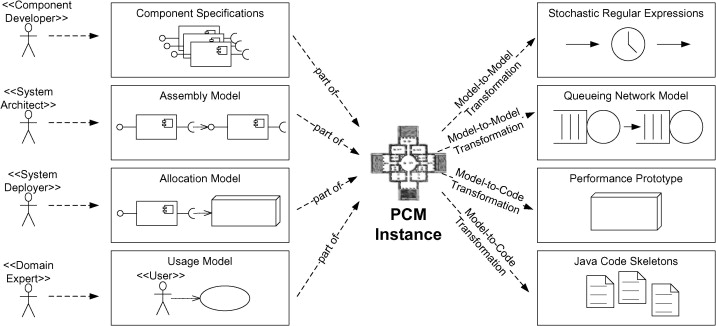
\includegraphics[width=15cm]{palladio-cbse-process}
  \caption[Instancia de un modelo PCM]{Instancia de un modelo PCM. Tomado de \protect\cite{Becker:2009:PCM:1458724.1458819}}
  \label{fig:pcm-instance}
\end{figure}

\begin{itemize}
    \item \textbf{Especificaciones de componentes} son descripciones abstractas y paramétricas de los componentes de software. En las especificaciones de software se proporciona una descripción del comportamiento interno del componente así como las demandas de sus recursos en RDSEFFs (\emph{Resource Demanding Service EFFect specifications}) utilizando una sintaxis similar a los diagramas de actividad de UML.
    \item \textbf{Un modelo de ensamblaje} (\emph{assembly model}) especifica qué tipo de componentes se utilizan en una instancia de aplicación modelada y si las instancias del componente se replican. Además, define cómo las instancias del componente se conectan representando la arquitectura de software.
    \item El entorno de ejecución y los recursos, así como la instalación (\emph{deployment}) de instancias de componentes para dichos contenedores de recursos se definen en un \textbf{modelo de asignación} (\emph{allocation model}).
    \item El \textbf{modelo del uso} especifica la interacción de los usuarios con el sistema utilizando una sintaxis similar al diagrama de actividades de UML proporcionando una descripción abstracta de la secuencia y la frencuencia en que los usuarios activan las operaciones disponibles en un sistema.
\end{itemize}

Un modelo PCM abstrae un sistema de software a nivel de arquitectura y se anota con consumos de recursos que fueron medidos previamente u otros que son estimados. El modelo puede entonces ser usado en transformaciones de modelo-a-modelo o modelo-a-texto a un modelo de análisis en particular (redes de colas o simulación de código) que puede ser analíticamente resuelto o simulado para obtener resultados sobre el rendimiento y predicciones del sistema modelado. Los resultados del rendimiento y las predicciones pueden ser utilizadas como retroalimentación para evaluar y mejorar el diseño inicial, permitiendo así una evaluación de calidad de los sistemas de software en base a un modelo\cite{Noorshams2015_1000046750}.


\subsubsection{Modelado de Arquitecturas de Software con \emph{Descartes Modeling Language}} 
El \emph{Descartes Modeling Language} (DML) es un lenguaje de modelado a nivel de arquitectura utilizado para describir calidad de servicio (\emph{QoS} por sus siglas en inglés) y aspectos relacionados con la gestión de recursos de sistemas de información dinámicos, infraestructuras y servicios. DML distingue explicítamente diferentes tipos de modelos que describen el sistema y sus procesos de adaptación desde un punto de vista técnico y lógico. Juntos, estos diferentes tipos de modelos forman una instancia DML. La idea detrás del uso de estos modelos es separar el conocimiento acerca de la arquitectura del sistema y el comportamiento de su rendimiento (aspectos técnicos) del conocimiento de los procesos de adaptación del sistema (aspectos lógicos)\cite{KoBrHu2014-TechReport-DML}.

\begin{figure}[h]
  \centering
  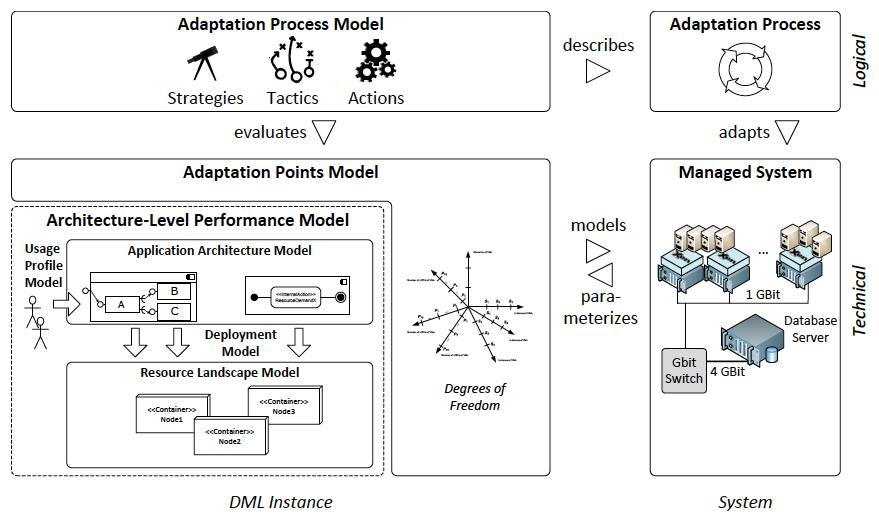
\includegraphics[width=16cm]{dml-instance}
  \caption[Relación de los diferentes modelos de una instancia DML y el sistema]{Relación de los diferentes modelos de una instancia DML y el sistema. Tomado de \protect\cite{KoBrHu2014-TechReport-DML}}
  \label{fig:dml-instance}
\end{figure}

La figura \ref{fig:dml-instance} muestra la relación de los diferentes modelos que son parte de una instancia DML, el sistema gestionado (\emph{managed system}) y el proceso de adaptación del sistema (\emph{adaptation process}). En la esquina inferior derecha de la figura \ref{fig:dml-instance}, se ve el sistema, el cual es gestionado por un proceso de adaptación, mostrado en la esquina superior derecha de la figura \ref{fig:dml-instance}. En la esquina inferior izquierda de, se muestran modelos que reflejan los aspectos técnicos del sistema. Esos aspectos son los recursos de hardware y su distribución (\emph{resource landscape model}), los componentes de software y el comportamiento relevante al rendimiento (\emph{application architecture model}), la instalación de componentes de software en el hardware (\emph{deployment model}), el comportamiendo del uso y las cargas de trabajo de los usuarios del sistema (\emph{usage profile model}) y los grados de libertad del sistema que pueden ser empleados para la adaptación del sistema en ejecución (\emph{adaptation points model}). Por encima de estos modelos (esquina superior izquierda de la figura \ref{fig:dml-instance}) se muestra el modelo de proceso de adaptación que especifica un proceso de adaptación que describe cómo el sistema se adapta a cambios en su ambiente. El proceso de adaptación aprovecha las técnicas de predicción de rendimiento en línea para razonar sobre posibles estrategias, tácticas y acciones de adaptación.
 
\subsection{Computación en nube}
La computación en la nube ha traído consigo nuevos estilos en la forma en cómo se desarrolla y se pone en producción el software. Esto motivado por ... \textbf{[EXTENDER]}


\subsection{Trabajos relacionados}

\subsubsection{Ingeniería de rendimiento de software en aplicaciones en la nube}

El estilo de arquitectura basado en microservicios es uno de los que ha logrado ganar mayor adopción y popularidad dentro de la comunidad de desarrolladores. Los microservicios, son una arquitectura de software que involucra la construcción y entrega de sistemas que se caracterizan por ser servicios pequeños, granulares, independientes y colaborativos \cite{10.1007/978-3-319-62636-9_11}. Con respecto a SPE y microservicios se reporta que existen muchos retos en investigación que han sido poco o nada abordados. 

En \cite{Heinrich:2017:PEM:3053600.3053653} se planean el monitoreo, pruebas y modelado del rendimiento como las tres áreas en donde se carece de investigación y desarrollo de SPE y microservicios. Se argumenta que aún hace falta de enfoques de SPE que tomen en cuenta las particularidades de los microservicios. Aderaldo et al.\cite{7968049} señala una falta de investigación empírica repetible sobre diseño, desarrollo y evaluación de aplicaciones de microservicios y que esto dificulta la evaluación de este tipo de aplicaciones ya que se cuenta con muy pocas aplicaciones y arquitecturas de referencia, así como de cargas de trabajo que contribuyan a caracterizar el comportamiento las mismas.

El reporte de \cite{DBLP:journals/corr/BrunnertHWDHHHJ15} también proporciona un listado de los retos asociados con microservicios y SPE, haciendo énfasis en actividades de SPE relacionadas con la integración de actividades de desarrollo y de operaciones de puesta en producción y mantenimiento del software. Se argumenta que a pesar del alto nivel de adopción de prácticas de integración continua, entrega continua y DevOps de la comunidad de ingeniería de software, ninguna toma en cuenta aspectos relacionados con el rendimiento. Otros estudios, como el llevado a cabo en \cite{7930195}, indican que uno de los atributos de calidad que ha recibido mayor atención en la investigación en microservicios es el de la eficiencia del rendimiento pero vista mayoritariamente desde el punto de vista de la escalabilidad y mantenibilidad del código de los microservicios y su instalación.

\textbf{[INCLUIR ESTUDIOS EN DONDE SI SE HA HECHO INVESTIGACION DE SPE Y MICROSERVICIOS?]}

\subsubsection{\emph{Serverless y Function-as-a-Service}}
FaaS es un área de lo que hoy se conoce como computación sin servidores o \emph{serverless computing}. Amazon.com, uno de los principales propulsores de esta tendencia define \emph{serverless} como una tecnología la cual permite construir y ejecutar aplicaciones y servicios sin necesidad de pensar en los servidores. Las aplicaciones \emph{serverless} no requieren de aprovisionamiento, escalamiento y administración de ningún servidor. Se puede construir con ella casi cualquier tipo de aplicación o servicio, y todo lo que se requiere para ejecutar y escalar la aplicación con alta disponibilidad es gestionado por el proveedor del servicio\cite{amazon:serverless-definition}. 

FaaS se refiere a un tipo de aplicación \emph{serverless} en donde la lógica del lado del servidor es escrita por un desarrollador pero, a diferencia de arquitecturas tradicionales, esta se ejecuta en contenedores de cómputo que no mantienen estado, son activados por medio de eventos, son efímeros (pueden durar solo una invocación) y son totalmente administrados por un tercero\cite{mike-roberts-serverless}.

Cabe destacar que aunque el término \emph{serverless} ha llegado a ser utilizado para referirse de forma directa a plataformas FaaS, hoy en día la aplicaciones de \emph{serverless computing} abarcan otros tipos de servicios como almacenamiento, mensajería, análisis de datos, seguridad, entre otros.

Los investigadores han empezado a describir y analizar FaaS a través de encuestas y experimentos\cite{DBLP:journals/corr/BaldiniCCCFIMMR17,Crane:2017:ESA:3121050.3121086,8360324}, y también por análisis económicos\cite{7515686,8247460}, sin embargo se reporta que aún no se conoce mucho acerca de SPE en FaaS. En \cite{Heinrich:2017:PEM:3053600.3053653} se menciona que al igual que con microservicios, FaaS también requiere de nuevas estrategias de modelado para capturar el comportamiento del código bajo estas infraestructuras. Los modelos de rendimiento tradicionales basados en en la noción de máquinas independientes podría ser inadecuado. 

En van Eyk et al.\cite{vanEyk:2018:SRC:3185768.3186308} se presenta un informe confeccionado por el \emph{Standard Performance Evaluation Corporation RG Cloud Group\footnote{\url{https://research.spec.org/working-groups/rg-cloud.html}}} (SPEC RG Cloud) sobre desafíos asociados a rendimiento en arquitecturas FaaS. Los principales temas son los que tienen que ver con evaluación y comparación de plataformas de FaaS, reducción del \emph{overhead}, políticas de \emph{scheduling}, la relación costo-rendimiento de una función y predicción del rendimiento. El informe también señala que actualmente muchas de las tareas de evaluación y pruebas para FaaS se vuelven complicadas porque no se cuenta con aplicaciones, arquitecturas ni cargas de trabajo de referencia, este es un trabajo que pretende abordar el SPEC RG Cloud. Con respecto a predicción del rendimiento, se indica que la aplicación de modelos de rendimiento de sistemas de software tradicionales en FaaS trae nuevos retos como la brecha de información (\emph{information gap}) y el rendimiento de una función en particular. La brecha de información significa que el usuario de FaaS no está consciente de los recursos de hardware en los que las funciones son ejecutadas, mientras que por otro lado, la plataforma de FaaS no tiene información acerca de los detalles de la implementación de la función. Tal y como en las aplicaciones tradicionales, la entrada (tamaño, estructura y contenido) influyen en el rendimiento de una función, el hecho de tener una infraestructura oculta hace necesario encontrar nuevos modelos que logren predecir de forma precisa el rendimiento de una función. Técnicas de modelado desarrolladas para sistemas de software se podrían aprovechar para FaaS, como por ejemplo modelado y simulación de arquitecturas de software basados en componentes. 

La aplicación de \emph{serverless computing} es una área activa de desarrollo. En trabajos previos \cite{7979855,hendrickson2016serverless} se han estudiado arquitecturas alternativas de \emph{serverless computing} con el fin de explotar aspectos de rendimiento y/o abordar retos técnicos que otras plataformas no han hecho. También se han investigado arquitecturas para recuperación de información\cite{Crane:2017:ESA:3121050.3121086} y \emph{chatbots}\cite{Yan:2016:BCS:3007203.3007217} utilizando plataformas \emph{serverless}. Muchas otras aplicaciones se han venido desarrollando en campos como \emph{Machine Learning}, seguridad, Internet de las cosas, procesamiento de voz, sistemas de archivos, etc, y son solo una muestra del potencial de esta tecnología. Pese a este potencial, también se reporta que aún no se sabe mucho acerca de cuáles herramientas se usan para producir, instalar y ejecutar funciones\cite{Spillner:2017:PTS:3147213.3149452}. En \cite{8360324} se examinan factores qué pueden influir en el rendimiento de plataformas de \emph{serverless computing}. De acuerdo a esto se logran identificar cuatro estado de una infraestructura \emph{serverless}: \emph{provider cold}, \emph{VM cold}, \emph{container cold}y \emph{warm}. Además demuestra cómo el rendimiento de los servicios puede llegar a variar hasta 15 veces según estos estados.


\chapter{Definición del problema}
\label{cap:problema}
Se carece de modelos de rendimiento que contribuyan a caracterizar el comportamiento de funciones en la nube alojadas en plataformas FaaS bajo distintas cargas de trabajo. Contar con tales modles permitiría validar si las funciones en la nube pueden cumplir criterios de calidad de servicio especificados.

%para de esta forma tener la capacidad de validar si estas pueden llegar a cumplir los criterios de calidad de servicio establecidos.

En las plataformas FaaS en las que se ejecutan funciones en la nube, la infraestructura tecnológica subyacente se oculta por completo de los desarrolladores y diseñadores. El conocimiento de la influencia de esta infraestructura y su configuración es vital para que los arquitectos de software puedan obtener predicciones significativas del comportamiento de una función pues, al omitirse la influencia que esta tiene, puede conducir a la generación de predicciones erróneas con respecto del rendimiento de una función. Una función que reporte tiempos de respuesta sumamente prolongados o bien la utilización de significativas cantidades de recursos puede generar grandes costos económicos y hasta llegar a ser rechazada por la plataforma FaaS.

%Las decisiones que hayan sido tomadas con poca información durante las etapas de diseño usualmente son muy difíciles de alterar y pueden impactar de forma negativa en los niveles requeridos de rendimiento de un sistema una vez que este ha sido puesto en producción. Es por esto que los arquitectos y diseñadores necesitan contar con la habilidad de predecir el rendimiento de una función trabajando a partir de diseños abstractos sin tener acceso a la implementación completa de la aplicación.

\chapter{Justificación}
\label{cap:justificacion}
\section{Innovación}
Los aspectos más novedosos que se aportarán esta tesis serán:
\begin{enumerate}
    \item Proponer un método mediante el cual se pueden obtener estimaciones del rendimiento de una función en la nube
    \item El uso de modelado y simulación basado en componentes para caracterizar el rendimiento de funciones en la nube en plataformas FaaS
    \item Proporcionar, a partir de lo anterior, un modelo del rendimiento de una función en la nube    
\end{enumerate}

Con respecto de (1), en \cite{vanEyk:2018:SRC:3185768.3186308} se reporta que la predicción del rendimiento es uno de los principales retos de investigación en plataformas FaaS y que no se cuenta con modelos de rendimiento que consideren las características de FaaS. Esto abre la posibilidad de explorar la aplicabilidad de técnicas conocidas de modelaje de rendimiento en sistemas de software a nuestro dominio de problema. 

El modelado y simulación de arquitecturas de software basadas en componentes (2), representa una alternativa atractiva para abordar este problema, esto porque es un enfoque en donde hay una comunidad de investigación y desarrollo activa que ha logrado generar diferentes tipos de herramientas para la estimación del rendimiento de un sistema informático. 

La obtención de un modelo de rendimiento de una función en la nube (3), representaría un aporte relevante para SPE y FaaS porque significaría que existe una forma por medio de la cual evaluar el comportamiento de una función sin que esta esté necesariamente instalada en una plataforma FaaS y además permitiría que cambios futuros que necesite esa función puedan ser modelados \emph{a priori}, simularlos y obtener predicciones del impacto de los cambios.



\section{Impacto}
En distintos reportes sobre el estado de tecnologías \emph{serverless} en la industria \cite{dzone-cloud-2018,rightscale-2018,digital-ocean-2018,pivotal-june-2018} se señala que la adopción de este tipo de tecnologías va en franco aumento. En \cite{rightscale-2018} se reporta una tasa de crecimiento del 25\% en su adopción con respecto al 2017. Cloud Foundry Foundation \cite{pivotal-june-2018} indica que el 2017 ``la mayoría'' de sus encuestados no estaban usando tecnologías \emph{serverless} mientras que para el 2018, solamente 43\% \textbf{no} lo estaba haciendo. En el informe anual del estado de tecnologías en la nube de DZone\cite{dzone-cloud-2018} se notó un incremento del 14\% con respecto al 2017 en el uso de tecnologías \emph{serverless}.

Pese a que los niveles de adopción de esta tecnología van en aumento, estos mismos reportes señalan incovenientes tales como:
\begin{enumerate}
    \item Se tiene que depender de los niveles de servicio un proveedor
    \item Dificultad para monitorear y depurar
    \item Preocupación por parte de los desarrolladores por el ``cómo funciona'' la función en la plataforma FaaS: ¿se estarán asignando los recursos adecuados para mi función en la plataforma FaaS? ¿Cómo y cuándo se hace?
    \item Límites de tiempo de espera: dependiendo del tiempo de ejecución una función en la nube podría llegar a ser cancelada por la propia plataforma FaaS
\end{enumerate}

Lo anterior refleja que aún existe una especie de ``área gris'' alrededor del uso de las tecnologías \emph{serverless} y en particular funciones en la nube. Esto es lo que van Eyk et al.\cite{vanEyk:2018:SRC:3185768.3186308} llama brecha de la información: el usuario de FaaS no está consciente de los recursos de hardware en los que las funciones son ejecutadas, mientras que por otro lado, la plataforma de FaaS no tiene información acerca de los detalles de la implementación de la función.

Analizar el rendimiento de una función en la nube y obtener un modelo de este contribuiría a tener un mejor entendimiento de esta tecnología y de cómo esta es gestionada por la plataforma FaaS. Esto permitiría a los arquitectos y diseñadores tener mayor control sobre los cambios en una función para que esta no solamente pueda cumplir con los requerimientos de calidad de servicio sino que también al ser \emph{serverless} un servicio que se cobra por demanda colaboraría a reducir gastos, ya que una función que tenga un tiempo de ejecución menor generá menores costos por el uso de la plataforma FaaS.

\section{Profundidad}
Para lograr obtener un modelo de rendimiento de una función en la nube se plantean las siguientes actividades:
\begin{itemize}
    \item Diseño e implementación de un caso de uso de referencia de una función en la nube 
    \item Obtención un modelo:
    \begin{itemize}
        \item Realizar pruebas de carga sobre la función en la nube seleccionada
        \item Obtener métricas asociadas al rendimiento a partir de bitácoras de ejecución de la función
        \item Utilizar las métricas obtenidas para suministrarlas como entrada a una herramienta de extracción de modelos de rendimiento. La herramienta generará como resultado un modelo de rendimiento
    \end{itemize}
    \item Diseñar experimentos y ejecutar simulaciones sobre el modelo obtenido con el fin de validar las estimaciones o determinar si es necesario calibrar el modelo
    
%     si los resultados obtenidos logran estimaciones adecuadas de la ejecución de la función o si por el contrario se necesita calibrar el modelo.
\end{itemize}

%\subsection{Implementación de un caso de uso de referencia de una función en la nube} 
%Se seleccionará un caso de uso en el cual el uso de una función en la nube haya mostrado ser una solución adecuada. Una vez identificado este caso de uso, se implementará la función y se instalará en una plataforma FaaS.

%\subsection{Obtención de un modelo} 
%Las plataformas FaaS proporcionan bitácoras en donde se registran métricas asociadas a la ejecución de la función en la nube. Se planea entonces ejecutar pruebas sobre la función en la nube bajo diferentes cargas de trabajo y de estar forma poder contar con una bitácora(s) con todas las métricas obtenidas durante el tiempo que tomó la ejecución de las pruebas. 




\chapter{Hipótesis}
\label{cap:hipotesis}
En el modelo FaaS, la infraestructura tecnológica subyacente se oculta por completo de los diseñadores y desarrolladores, asimismo, la duración de la ejecución de una función en la nube determina el costo del servicio: entre mayor sea la duración, mayor será el costo y viceversa. Si bien se han realizado estudios \cite{8360324} para evaluar factores que influyen en el rendimiento de servicios basados en computación \emph{serverless}, el modelado del rendimiento de este tipo de aplicaciones se sigue presentando como un reto de investigación \cite{Heinrich:2017:PEM:3053600.3053653}. El modelado del rendimiento ha ganado considerable atención en la comunidad de ingeniería de rendimiento en las pasadas dos décadas, principalmente en sistemas de software basados en componentes \cite{Koziolek:2010:PEC:1808359.1808729}. Al finalizar y alcanzar los objetivos de la investigación se podrá contar con un marco de referencia que permitirá:
\begin{itemize}
    \item Tener una función en la nube que servirá como prueba de concepto funcional para la evaluación del rendimiento
    \item Contar un método mediante el cual se pueda analizar el rendimiento de una función en la nube por medio de modelado y simulación.
\end{itemize}


Una vez alcanzados los objetivos, será posible responder a la pregunta:


\textbf{¿Es posible estimar el rendimiento de una función en la nube por medio de modelado y simulación basados en componentes?}

\chapter{Objetivos}
\label{cap:objetivos}
\section{Objetivo general}
Diseñar un método para modelar el rendimiento de funciones en la nube alojadas en plataformas \emph{Function-as-a-Service} por medio del modelado y la simulación basados en componentes, con el fin de evaluar los factores que pueden influir en su comportamiento. 

\section{Objetivos específicos}
\begin{enumerate}
    \item Revisar el estado del arte de trabajos relacionados con enfoques de predicción y medición del rendimiento en sistemas de software como servicio
    \item Sintetizar un caso de uso de una función en la nube considerada como de referencia, con el propósito de analizar su comportamiento
    \item Elaborar, conforme a un diseño experimental, pruebas de rendimiento sobre el caso de uso seleccionado a fin de obtener datos base
    \item Analizar los datos experimentales mediante herramientas de extracción de modelos de rendimiento de software 
%    \item Realizar experimentos sobre la función en la nube de referencia con herramientas de modelado y análisis de rendimiento de sistemas informáticos     
    \item Proponer y validar modelos de rendimiento a partir de los experimentos realizados 
%    \item {\Huge **}Validar experimentalmente el modelo planteado        
    \item Formular una guía metodológica para dar a conocer aspectos de rendimiento en funciones en la nube a partir de la experiencia obtenida
   
    
%    \item \textbf{[CONSULTAR]} Comparar la solución obtenida con otra plataforma/lenguaje de programación, etc
\end{enumerate}

\chapter{Alcance}
\label{cap:alcance}
El estudio propuesto comprende:
\begin{itemize}
    \item Es estudio de los factores que pueden influir en el rendimiento de un caso de uso de una función en la nube bajo una plataforma FaaS en particular. Se espera que a partir de la experiencia recolectada, este trabajo podría ser replicado en otras funciones en la nube bajo otras plataformas FaaS.
    \item La propuesta de un modelo de rendimiento que permita la simulación de la ejecución de una función en la nube y obtener a partir de esta, estimaciones del tiempo de respuesta de la ejecución de la función.
\end{itemize}


El estudio propuesto \textbf{no} comprende:
\begin{itemize}
    \item El modelado y/o simulación de toda una plataforma FaaS.
    \item La realización de ningún modelo y/o estudio de los aspectos económicos asociados a la ejecución de una función en la nube.
    \item Estudiar el rendimiento de funciones en la nube que mantengan alguna relación y/o dependencias entre sí (orquestación de funciones)
    
\end{itemize}


\chapter{Entregables}
\label{cap:entregables}
\section[Revisión de literatura]{Revisión de literatura\\\small{Alineado con objetivo específico 1}}
Se pretende identificar los resultados de otros estudios relacionados con el modelado de rendimiento de software, así como retos y oportunidades de investigación que existan en esta área. Las preguntas de investigación inicialmente propuestas son las siguientes:
\begin{itemize}
    \item[\textbf{PI1}] ¿Cuáles enfoques de predicción y medición del rendimiento en sistemas de software basados en componente se han propuesto?
    \item[\textbf{PI2}] ¿Cuáles enfoques de predicción y medición de rendimiento de software se han utilizado para aplicaciones en la nube?
    \item[\textbf{PI3}] ¿Qué retos y oportunidades existen con estos enfoques en la actualidad?
    \item[\textbf{PI4}] ¿Qué herramientas hay disponibles para el modelado de rendimiento de software?
\end{itemize}

\section[Implementación de caso de uso de función en la nube]{Implementación de un caso de uso de función en la nube\\\small{Alineado con objetivo específico 2}}

Identificar un caso de uso de que sea considerado como de referencia o ``bien conocido'' en donde las funciones en la nube hayan mostrado ser un buen candidato para su solución. Se procederá a implementar este caso de uso e instalarlo en una plataforma FaaS. Esta será la función que servirá como base para futuro análisis.

\section[Pruebas sobre el caso de uso]{Pruebas sobre el caso de uso\\\small{Alineado con objetivo específico 3}}

\subsection{Diseño experimental}
Planeamiento y definición de las variables por observar de las pruebas de carga.

\subsection{Pruebas de carga}
Diseño, ejecución y análisis de los resultados de las pruebas.

%\subsection{Resultados}


%\section[Medición del rendimiento del caso de uso]{Medición del rendimiento del caso de uso\\\small{Alineado con objetivo específico 3}}
%Al caso de uso identificado se le realizarán mediciones de su rendimiento por medio de diferentes cargas de trabajo. Esto permitirá conocer el comportamiento de la función y utilizar los resultados obtenidos en estas mediciones para contrastar resultados posteriores.

\section[Modelado y análisis del rendimiento de la función]{Modelado y análisis del rendimiento de la función\\\small{Alineado con objetivo específico 4}}
Se tomarán los datos generados de las pruebas anteriores para utilizarlas como entrada y, a partir de ellos, iniciar una labor de análisis y modelado.

\section[Modelo de rendimiento de la función en la nube]{Modelo de rendimiento de la función en la nube\\\small{Alineado con objetivo específico 5}}
A partir de la función propuesta, pruebas y análisis del rendimiento por medio de herramientas de modelado, se propone un modelo que logre caracterizar el comportamiento de la función.

\subsection[Simulaciones sobre el modelo propuesto]{Simulaciones sobre el modelo propuesto}
Para validar el modelo propuesto, se ejecutarán simulaciones sobre él y de esta forma determinar si los resultados de las simulaciones se corresponden con los obtenidos en las pruebas de rendimiento de la función.

\section[Guía metodológica]{Guía metodológica\\\small{Alineado con objetivo específico 6}}
Una vez realizado el estudio, se dará a conocer el método utilizado para estimar el rendimiento de una función en la nube. 

\chapter{Metodología}
\label{cap:metodologia}
\section{Selección de caso de uso}
Uno de los principales problemas de hacer ingeniería de rendimiento para software en la nube es que no existen aplicaciones de referencia las cuales hayan ganado popularidad o bien que su desarrollo se encuentre activo. A pesar de esto y de su reciente adopción, la industria ha empezado a reconocer casos de uso en donde aplicaciones \emph{serverless} encajan mejor. Amazon Web Services(AWS)\cite{serverless-architecture-patterns} reconoce cinco patrones de uso predominantes en su servicio AWS Lambda:
\begin{enumerate}
    \item Procesamiento de datos dirigidos por eventos
    \item Aplicaciones Web
    \item Aplicaciones móviles e Internet las cosas (IoT)
    \item Ecosistemas de aplicaciones \emph{serverless}
    \item Flujos de trabajo dirigidos eventos
\end{enumerate}
 
Uno de las aplicaciones más comunes en \emph{serverless} es desencadenar acciones luego de que ocurre un evento, por ejemplo luego de la modificación de un registro en una base de datos o bien luego de que se publica un mensaje en una cola de mensajería. Esto puede provocar que se active una función lambda que toma como entrada el evento recién publicado para su posterior procesamiento. Este estilo de caso de uso encaja bien en ambientes híbridos: ambientes en donde tecnologías \emph{serverless} se aprovechan para realizar funciones específicas dentro de una aplicación (o aplicaciones) más grande.

AWS ha publicado una serie de arquitecturas de referencias\cite{aws-lambda-ref-arch} para su plataforma FaaS, AWS Lambda. Dentro de estas arquitecturas se destaca el caso de uso de un manejador de imágenes (\emph{Image Handler})\cite{aws-lambda-image-handler}. 

\begin{figure}[h]
  \centering
  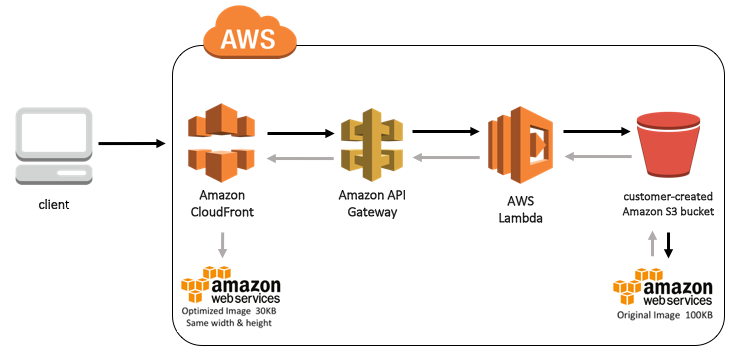
\includegraphics[width=15cm]{serverless-image-handler-architecture}
  \caption[Arquitectura del manejador de imágenes]{Arquitectura del manejador de imágenes. Tomado de \protect\cite{aws-lambda-image-handler}}
  \label{fig:serverless-image-handler-architecture}
\end{figure}

\subsection{\emph{Manejador de imágenes}} \label{sec:manejador-imagenes-1}
Sitios Web con imágenes grandes pueden experimentar tiempos de carga prolongados, es por esto que los desarrolladores proporcionan diferentes versiones de cada imagen para que se acomoden a distintos anchos de banda o diseños de página. Para brindar tiempos de respuesta cortos y disminuir el costo de la optimización, manipulación y procesamiento de las imágenes, AWS propone un manejador de imágenes \emph{serverless}, para que de esta forma se le pueda delegar este trabajo a una función lambda y a la plataforma FaaS.


A continuación se describe la arquitectura de la figura \ref{fig:serverless-image-handler-architecture}:
\begin{enumerate}
    \item Amazon CloudFront provee una capa de \emph{cache} para reducir el costo del procesamiento de la imagen
    \item Amazon API Gateway brinda acceso por medio de HTTP a las función Lambda
    \item AWS Lambda obtiene la imagen de un repositorio de Amazon Simple Storage Service (Amazon S3) y por medio de la implementación de la función se retorna una versión modificada de la imagen al API Gateway
    \item El API Gateway retorna una nueva imagen a CloudFront para su posterior entrega a los usuarios finales
\end{enumerate}

Cabe mencionar que en este contexto, una versión modificada de una imagen será cualquier imagen que haya presentado algún tipo de alteración con respeto a una imagen original como por ejemplo cambios de tamaño, color, metadatos, etc.

\subsection{Manejador de imágenes para SPE}
Para este estudio se propone implementar una variación del manejador de imágenes de la sección \ref{sec:manejador-imagenes-1}, que se muestra en la figura \ref{fig:serverless-image-handler-architecture-spe}.

\begin{figure}[h]
  \centering
  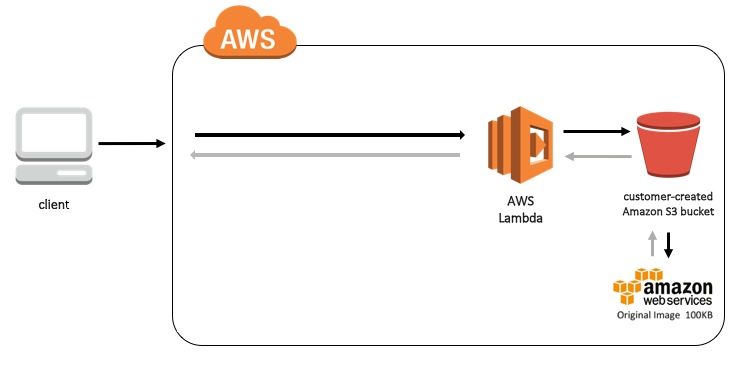
\includegraphics[width=15cm]{serverless-image-handler-architecture-spe}
  \caption[Arquitectura del manejador de imágenes propuesto para el estudio]{Arquitectura del manejador de imágenes propuesto para el estudio.}
  \label{fig:serverless-image-handler-architecture-spe}
\end{figure}

Se han dejado por fuerta intencionalmente el AWS CloudFront y el AWS API Gateway. La razón de esto es porque se pretende ejercitar la función Lambda directamentamente. Se implementará una función Lambda que entregue a partir de una imagen, otra con dimensiones diferentes. Por ejemplo si la imagen original mide 500 pixeles de ancho y alto, entregar una con dimensiones de 100 pixeles de ancho y alto. 

A la función Lambda se le realizarán pruebas con imágenes de entrada de distinto tamaño para evaluar su comportamiento bajo estos escenarios, particularmente del tiempo de respuesta de la función. Los resultados obtenidos a partir de estas pruebas van a servir como un punto de referencia para experimentos futuros. 

\chapter{Cronograma de actividades}
\label{cap:cronograma}
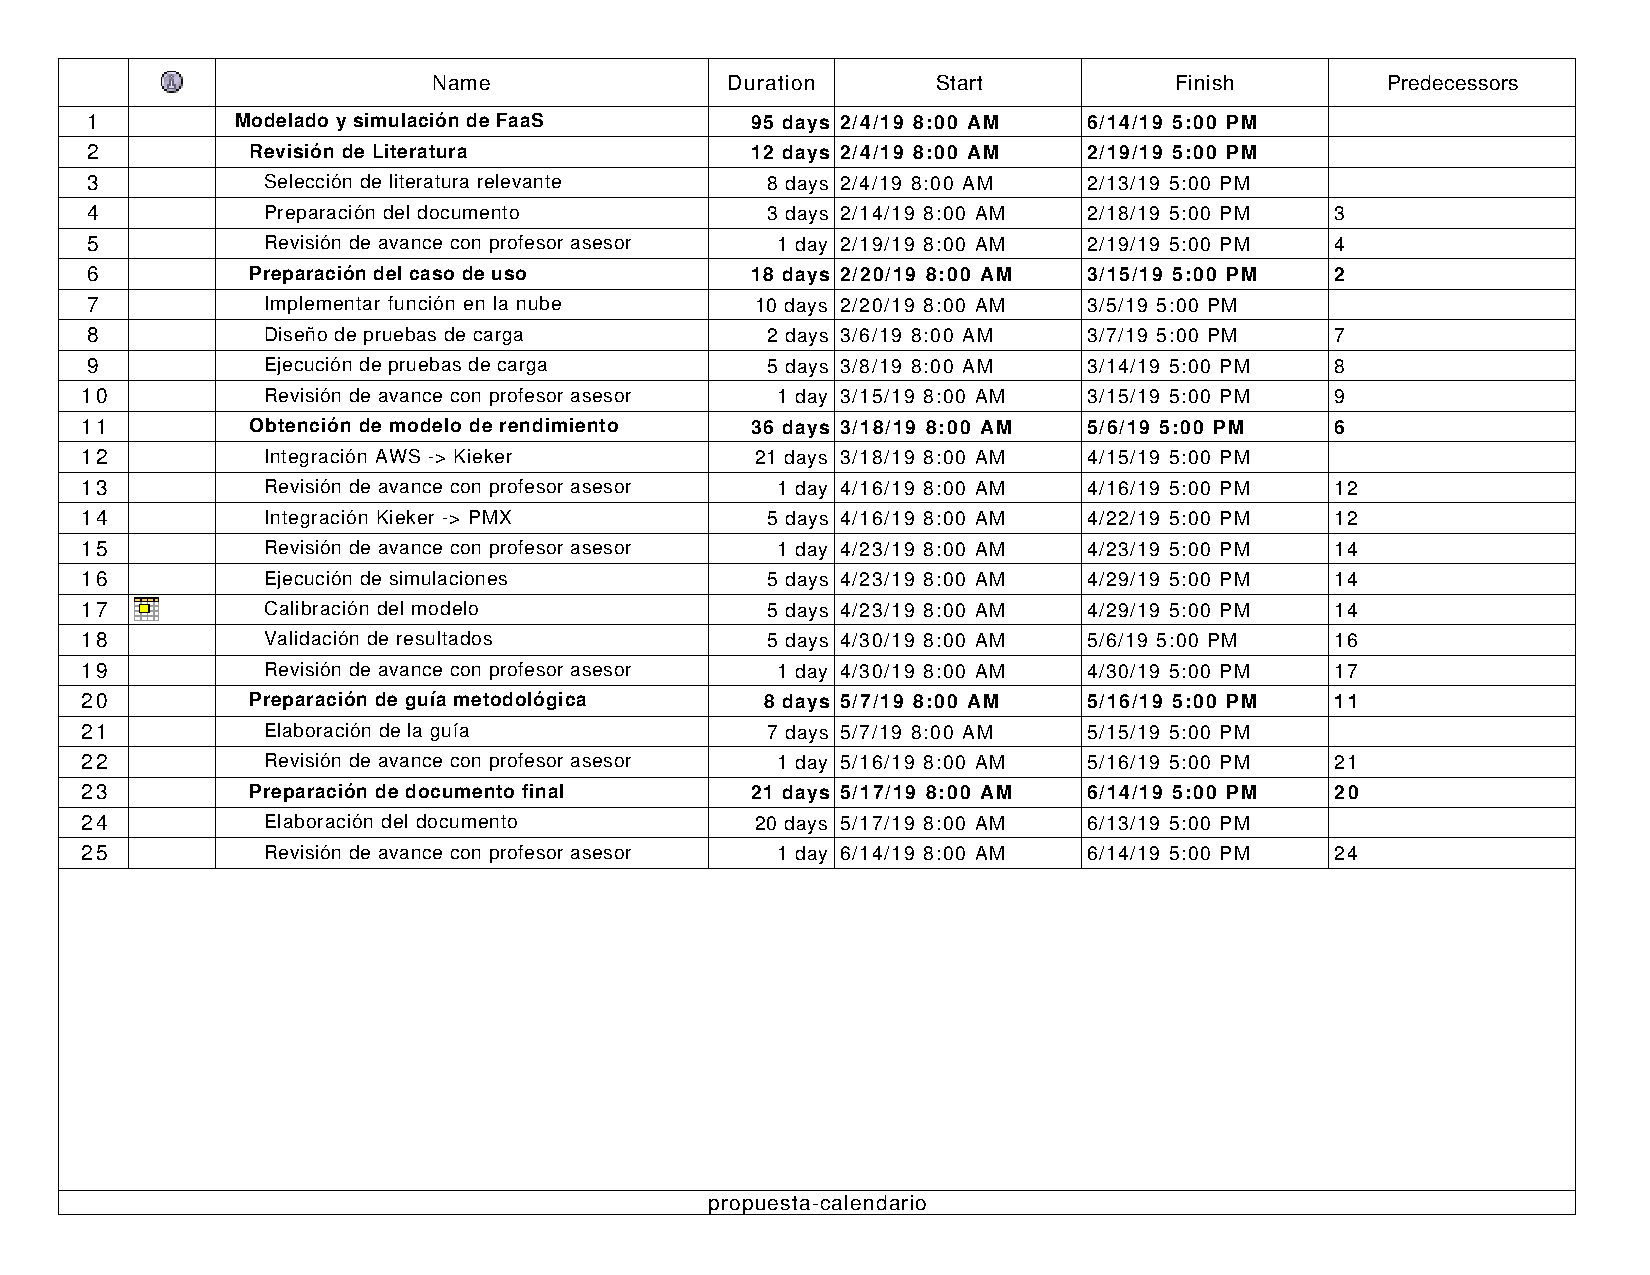
\includepdf[landscape, pages=1]{propuesta-calendario-spreadsheet}
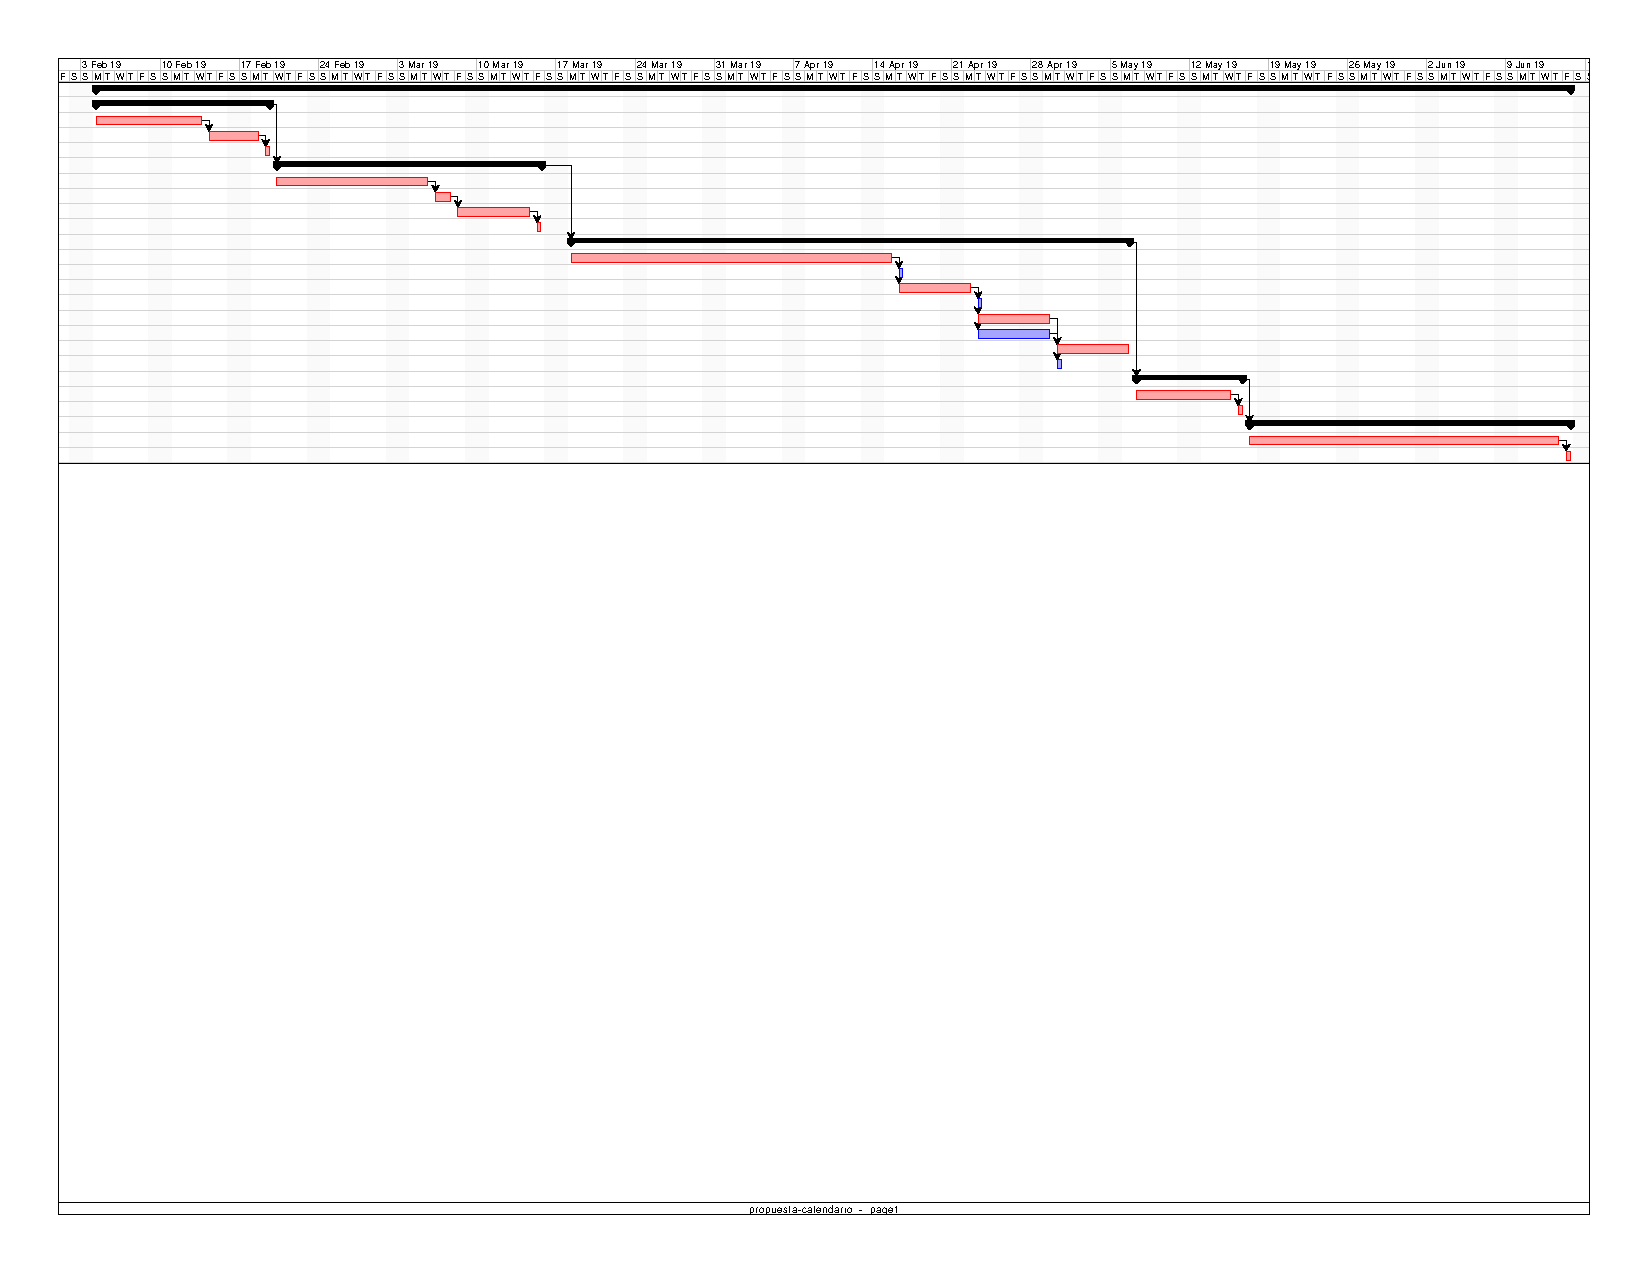
\includepdf[landscape, pages=1]{propuesta-calendario-gantt}

\addcontentsline{toc}{chapter}{Bibliografía}
\bibliographystyle{ieeetr}
\bibliography{referencias}

\end{document}
